\subsection{Description}
Tree-aggregate is a communication patten heavily used for Machine Learning algorithm in Spark (MLlib). 
In the traditional aggregation function in Spark, results of aggregation in all executor clusters are sent to the driver. 
That is why this operation suffers from the CPU cost in merging partial results and the network bandwidth limit.
Tree-aggregate is a communication pattern which overcomes these problems by breaking aggregate operation in multi-level represented like tree structure.

In our experiment, tree-aggregation algorithms are examined in multi-threading. This experiment is to evaluate the impact of having Arc (Atomic Reference Counting) as elements of vector. 
In Big Data mining tool, such as Spark, it generates intermediate objects from original source vector. In tree-aggregation, aggregated HashMap like data structure is created in each step or node. 
Acquisition of elements in source vector is required to perform this aggregation. There are several ways.

One way is deep-copy elements of vector. This solution allocated newly created objects by deep-copy. 
Aggregation is performed on copied objects, stores them in the data structure and sends it to next node. 
Deep-copy generates duplicates of objects in vector and aggregated data structure. 
This can lead to memory intensive moment when we need memory space for the duplicated objects in addition.

The other way is to get reference to the elements. Since an original source vector is deallocated after a local aggregation,
Simple reference to elements does not live long enough and allow the aggregation result to be sent to next node. 
Instead of simple borrowing, we need owner in the aggregation result. Reference Counting (Rc) in Rust is a way to have multiple owners to a value. 
Since our experiment is implemented in multithreading, Atomic Reference Counting (Arc) is used instead of Rc. With Arc, multiple ownership pointer can be 
possessed by different variables across multiple threads. Therefore a value is not deallocated until all of owners to it are dropped. 
This does not require extra memory allocation, because only acquisition of new ownership to value is needed. 
However, deletion of Arc type checks whether the value is still owned by other variables. 
This checking may be a overhead in algorithms where generate a lot of intermediate data structures, because deletion of the data structures occurs in frequent.

Two algorithms are implemented using the above two different methods and evaluated their runtime performance. 
The both algorithms perform tree-aggregation where runs seven nodes. 
Each node load Customer vector from disk and aggregate it by Customer last name. Once a node finishes aggregation, it sends result to parent node. 
After parent nodes receive aggregation results from all of its children nodes, it joins all aggregation results including its and sends next parent. 
One algorithm performs aggregation by deep-copying elements from source vector loaded from disk. In the other algorithm, each element of source vector 
is wrapped in Arc, and its reference is acquired while aggregation. 


\subsection{Result}

Figure shows runtime performance of two tree-aggregate algorithms. The runtime of algorithm with deep-copy is slower than algorithm with Arc for every vector size. 
This is result of overhead of deep-copy is larger than deletion of Arc. 

\begin{figure}[htb]
    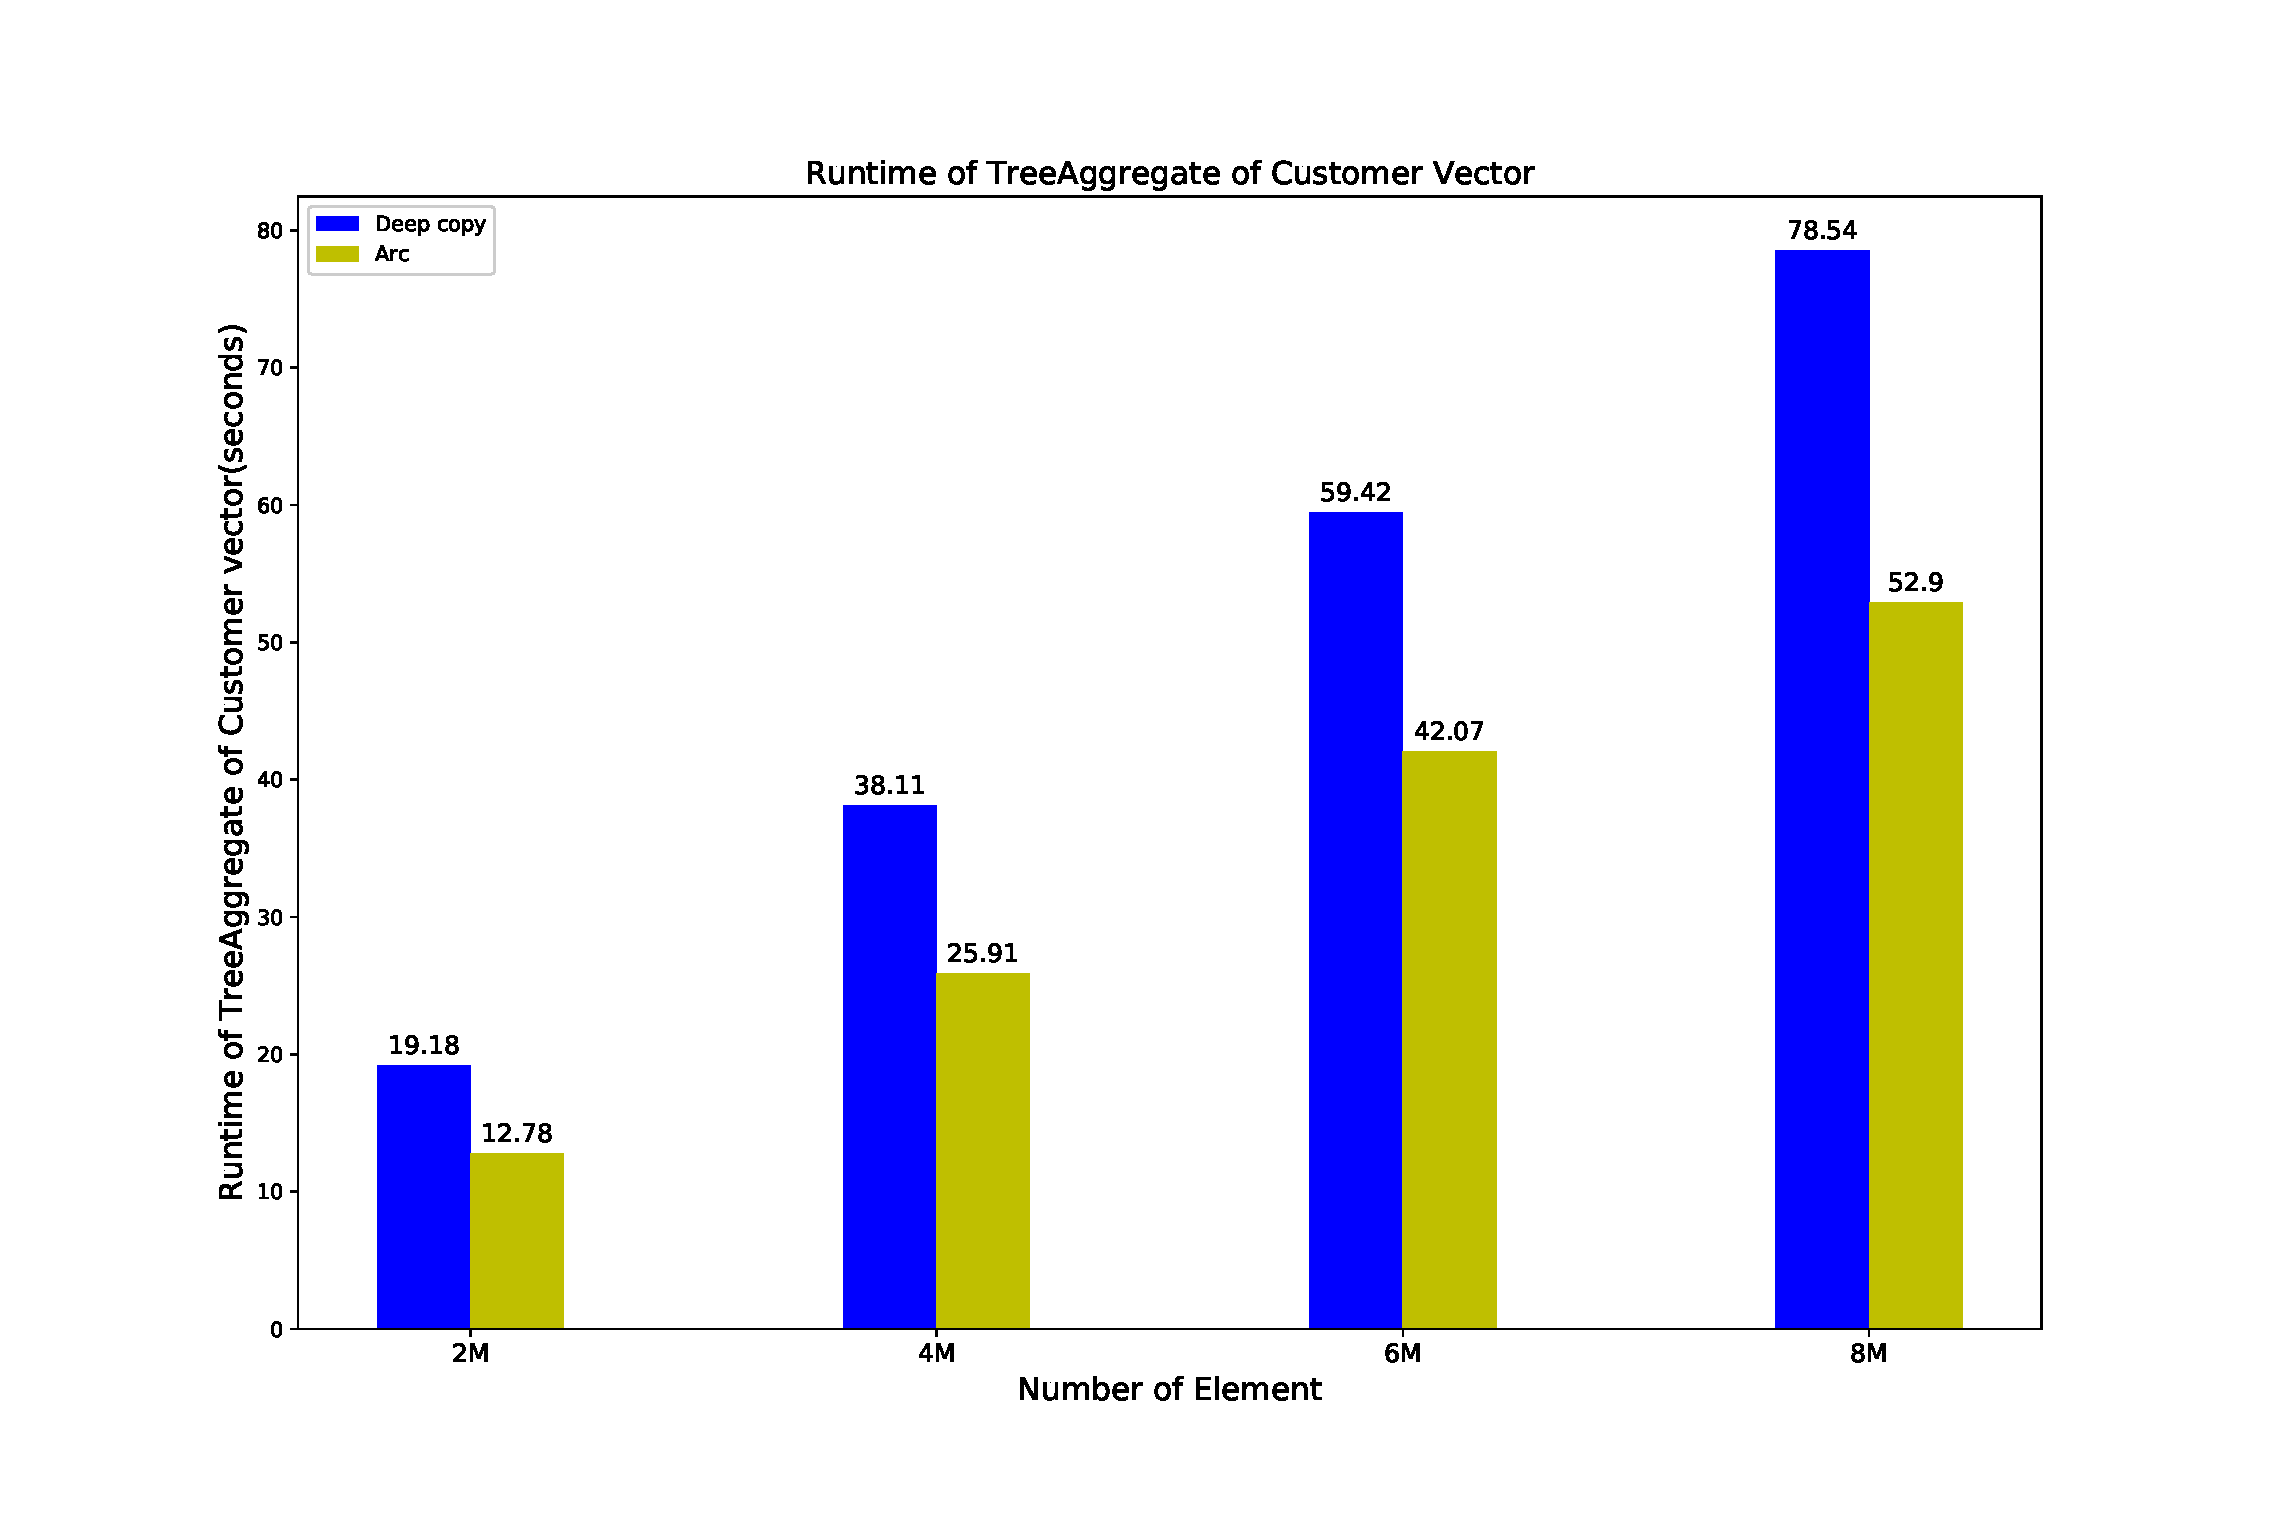
\includegraphics[width=15cm]{rust_tree_aggregate.eps}
    \caption{Runtime of Tree-aggregate algorithm}
    \label{fig:Sampling}
\end{figure}

\subsection{Discussion}
As we explained, Arc has overhead to be deleted because it has to check if the value is still referred. 
Even though the deletion of Arc is slow, deep copy of complex objects has more impact in deterioration of runtime performance. 
In the algorithm with deep copy, the elements of each partition in each node are deep-copied once during aggregation. 

If total number of elements are 1000000, the all of 1000000 elements are deep-copied once during execution. On the other hand, acquisition and deletion of Arc occurs several time for each element object.
First, acquisition of Arc of all elements in loaded vector happens during aggregation in each node and the loaded vector is deleted after the aggregation. 
Second, deletion of all elements in aggregated structures from children nodes and the node is occurs after joining these aggregated structures to single one. 

The result shows a deep-copy of Customer vector is computationally much more expensive than acquisition and deletion of Arc. 
This result suggests that having element objects in Arc is efficient than deep-copying element from original source vector in tree-aggregation algorithm 
where generates intermediate data structure. 